\documentclass[final]{beamer}

\mode<presentation> { \usetheme{Rochester} }
\setbeamersize{text margin left=0.6cm,text margin right=0.6cm}
\setbeamertemplate{navigation symbols}{}
\setbeamertemplate{headline}{
  \leavevmode
  \pgfsetfillopacity{0.7}
  %%\begin{beamercolorbox}[wd=\paperwidth*0.8,dp=2ex]{subsection in head/foot}
    \usebeamerfont{subsection in head/foot}
    \begin{columns}[T]
      \begin{column}{.75\paperwidth}
        \begin{beamercolorbox}[wd=\columnwidth,dp=2ex]{subsection in head/foot}
        \vskip4ex
        \begin{flushright}
          \usebeamercolor{title in headline}{
            \color{fg}\textbf{\huge{\pgfsetfillopacity{1} \inserttitle \hspace*{1cm} }}\\[1ex]
          }
          \usebeamercolor{author in headline}{
            \color{fg}\Large{\pgfsetfillopacity{1} \insertauthor \hspace*{1cm} }\\[1ex]
          }
          \usebeamercolor{institute in headline}{
            \color{fg}\Large{\pgfsetfillopacity{1}  \insertinstitute \hspace*{1cm} }\\[1ex]
          }
        \end{flushright}
        \vskip4ex
        \end{beamercolorbox}
      \end{column}

      \begin{column}{.25\paperwidth}
        \vskip0.5cm
        \begin{flushleft}
          
\includegraphics[width=.7\columnwidth]{figures/logo4.png}
        \end{flushleft}
        \begin{flushleft}
          
\includegraphics[width=.40\linewidth]{figures/logo2.pdf}
          
\includegraphics[width=.40\linewidth]{figures/logo3.png}
        \end{flushleft}
      \end{column}
    \end{columns}
    \vskip0cm
  %%\end{beamercolorbox}
%  \begin{beamercolorbox}[wd=\paperwidth]{section in head/foot}
%    \rule{0pt}{2pt}
%  \end{beamercolorbox}
}

%%\setbeamertemplate{footline}{
%%  \leavevmode
%%  \begin{beamercolorbox}[leftskip=1cm,rightskip=1cm]{subsection in head/foot}
%%    \usebeamerfont{section in head/foot}
%%    \vskip1ex
%%    \normalsize
%%    \insertinstitute
%%    \hfill
%%    \texttt{\correspondingAuthorEmail}
%%    \hfill
%%    \texttt{\website}
%%  \end{beamercolorbox}
  %\begin{beamercolorbox}[wd=\paperwidth]{section in head/foot}
    %\rule{0pt}{2pt}
  %\end{beamercolorbox}
%%}



\usepackage[english]{babel}
\usepackage[utf8]{inputenc}
\usepackage{amsmath,amsthm,amssymb,latexsym}
\usepackage{multirow}
\usepackage[orientation=portrait,size=a0,scale=1.15]{beamerposter}

\usebackgroundtemplate%
{
    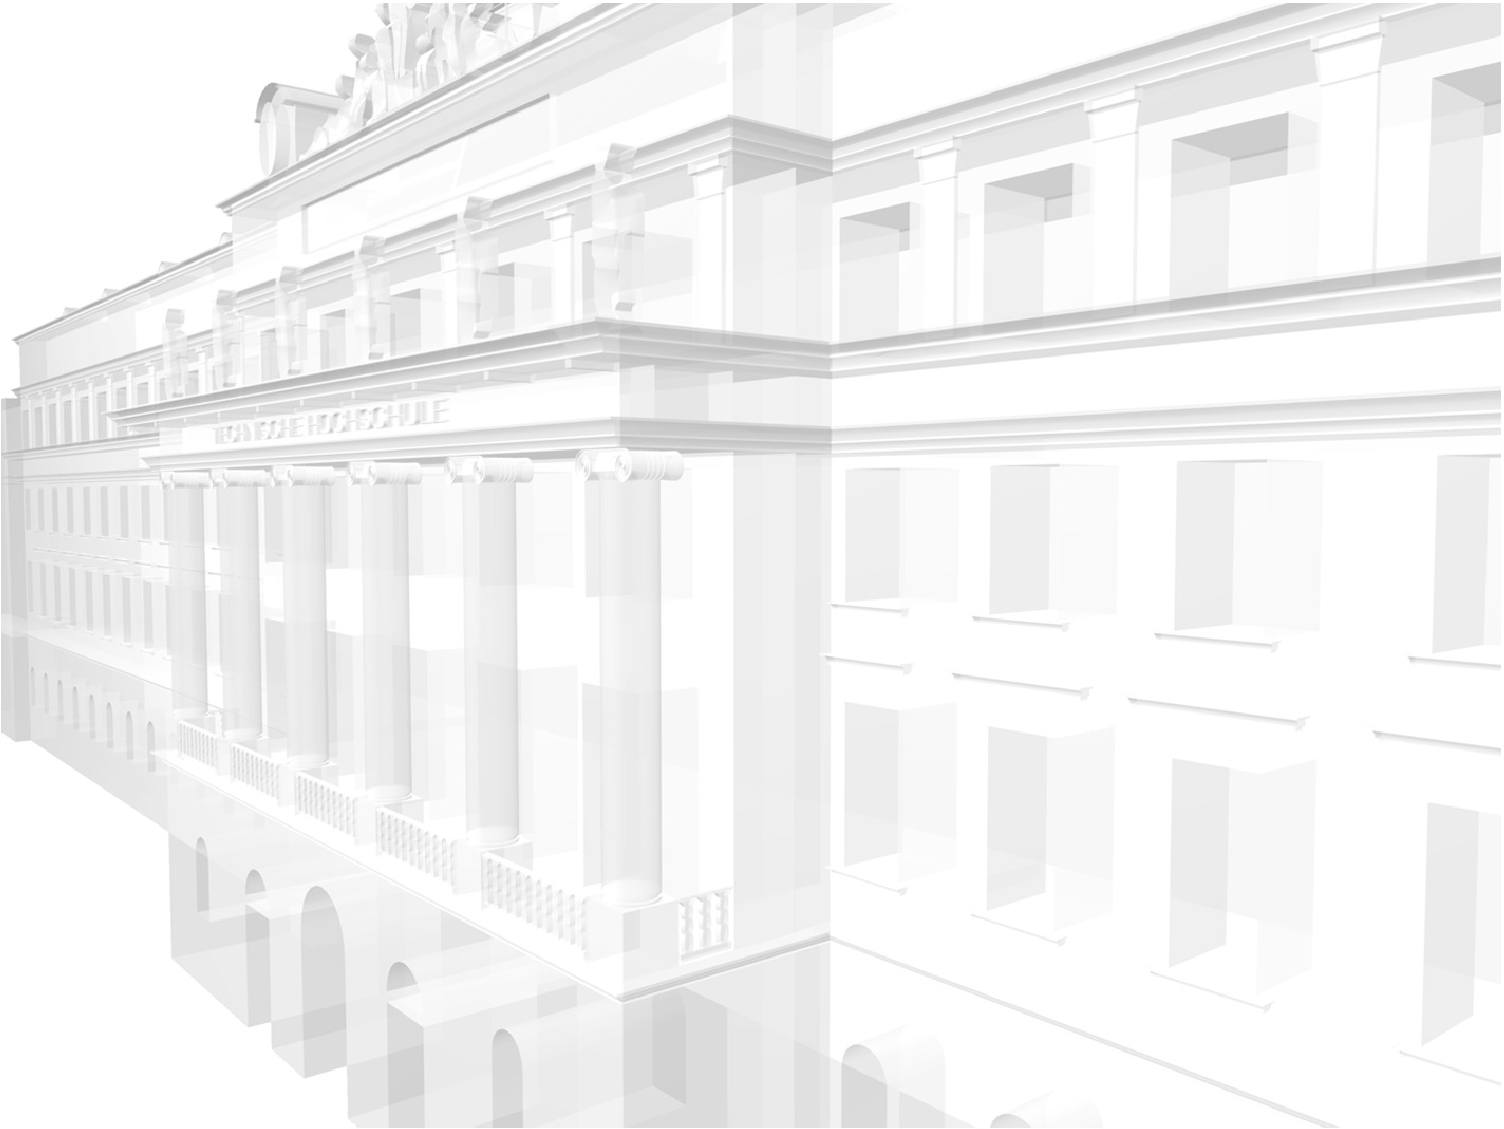
\includegraphics[width=\paperwidth,height=0.5\paperheight]{figures/TU_building.pdf}
}

\title{Towards driving Quantum Systems in cryogenic environments\hspace*{1cm} \\ with the Near-Field of Modulated Electron Beams}
\author{\underline{T. Spielauer$^{1}$}, M. Kolb$^{1}$, T. Weigner$^{1}$, J. Toyfl$^{1}$, G. Boero$^{2}$, P. Haslinger$^{1}$ }
\def\correspondingAuthorEmail{thomas.spielauer@tuwien.ac.at}
\def\website{}
\institute[]{
  {\small
  $^{1}$VCQ, Technische Universität Wien, Atominstitut, Stadionallee 2, 1020 Vienna, Austria; $^{2}$EPFL, BM 3110 Station 17, CH-1015 Lausanne, Switzerland
  }
}


\begin{document}
\begin{frame}[fragile]{}
  \pgfsetfillopacity{0.80}
  \begin{block}{\large Abstract}
    Coherent electromagnetic control of quantum systems is usually done by
    electromagnetic radiation - which does not permit addressing single site-selected
    quantum systems, especially in the microwave range. In our proof of concept
    experiment we want to couple for the first time the non-radiative electromagnetic
    near-field of a spatially modulated electron beam to a quantum system in
    a coherent way as has been proposed lately[1].  As the quantum system we
    use the unpaired electron spins of a free radical organic sample (Koelsch radical
    - $\alpha,\gamma$-Bisdiphenylene-$\beta$-phenylallyl) that is excited via the
    near-field of the aloof electron beam. The readout of the spin excitation
    resembles a classic continuous wave electron spin resonance experiment and is
    done inductively via a microcoil using a lock-in amplifier.

    The long term perspective of this experiment is the ability to coherently drive
    and investigate quantum systems in a spatial volume way below the diffraction
    limit of traditional electromagnetic wave based excitation schemes. The spatially
    confined excitation using an electron beam could also be realized within
    an electron microscope. Within the last year we have been able to improve
    the setup, couple the electron beam to the microcoil and reduce noise sources
    as well as started preparations to cool down the microcoil setup to cryogenic
    temperatures for enhanced signal to noise ratio.
  \end{block}
  \begin{columns}[T]
    \begin{column}{.49\linewidth}
      \begin{block}{\large The Quantum Klystron}
        We call our experiment the \textit{Quantum Klystron}, referencing an established
        technology, the Klystron.

        \begin{columns}
          \begin{column}{0.4\columnwidth}
              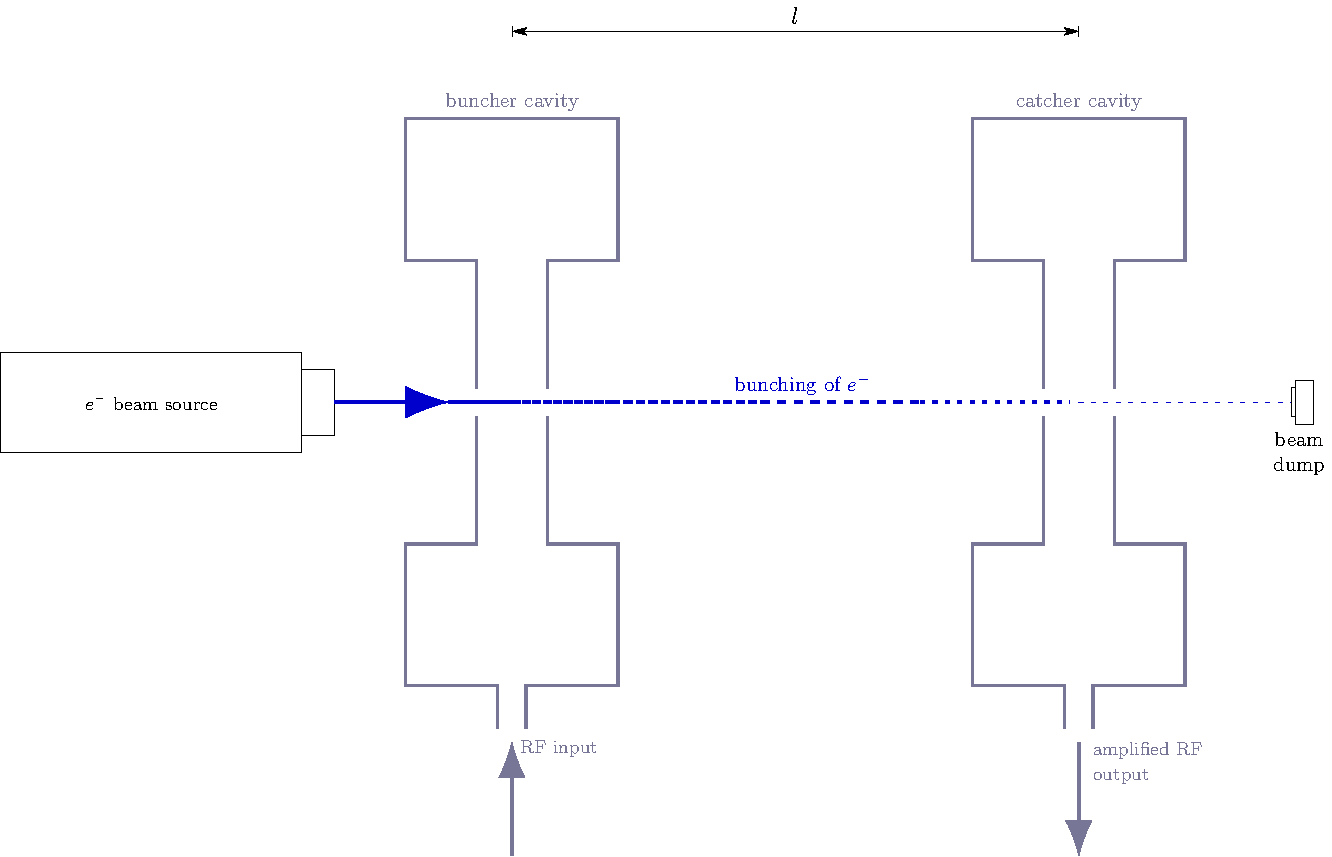
\includegraphics[width=\columnwidth]{figures/klystron.pdf}
          \end{column}
          \begin{column}{0.6\columnwidth}\begin{center}
              {\large \textbf{Klystron}}
            \end{center}

            \begin{itemize}
              \item Linear beam vacuum tube invented in 1935, used as RF and microwave amplifier
              \item Electrons are accelerated into a linear tube
              \item Velocity modulation happens in a buncher cavity by the input signal
              \item A density modulated charge carrier wave forms through driftspace
              \item Outcoupling is done via a catcher cavity
            \end{itemize}
          \end{column}
        \end{columns}
        \begin{columns}
          \begin{column}{0.4\columnwidth}
            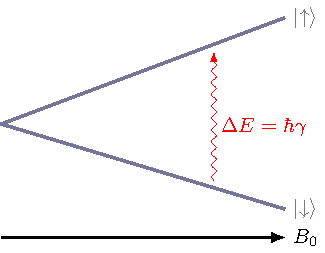
\includegraphics[width=\columnwidth]{figures/zeeman.pdf}
          \end{column}
          \begin{column}{0.6\columnwidth}
            \begin{center}
              {\large \textbf{Quantum Klystron}}
            \end{center}

            \begin{itemize}
              \item We replace catcher cavity with a 2 level quantum system
              \item Then we drive the system using the \textit{non-radiative electromagnetic near-field}
                    of an electron beam.
              \item Either modulate in
              \begin{itemize}
                  \item \textit{time domain} - bunching / density modulation
                  \item \textit{spatial domain} - deflection
              \end{itemize}
              \item Ability to draw arbitrary potentials (drive optical dipole, \\quadrupole, etc. transitions, spin systems, $\ldots$)
              \item High spatial resolution (de Broglie wavelength of modulated electron beam $\lambda_{DB}= 27.3 pm$, wavelength of a 202 MHz electromagnetic wave $\lambda=1.48m$)
            \end{itemize}
          \end{column}
        \end{columns}
      \end{block}

      \begin{block}{\large Electron spin resonance with electron beams}
        The experiment resembles an electron spin resonance experiment. In contrast to
        classic electron spin resonance setups where systems are excited using microwaves,
        we use the \textit{non-radiative electromagnetic near-field} of an electron beam.

        \begin{columns}
          \begin{column}{0.6\columnwidth}
            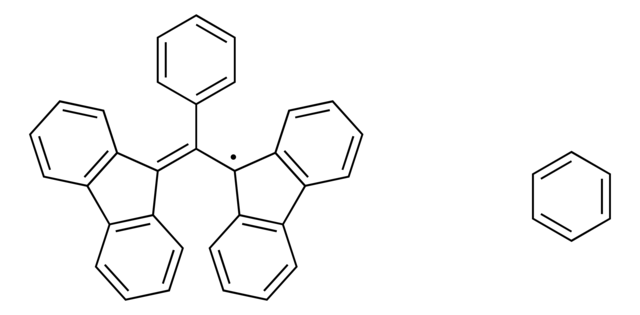
\includegraphics[width=0.67\columnwidth]{figures/bdpa.png}
          \end{column}
          \begin{column}{0.4\columnwidth}
            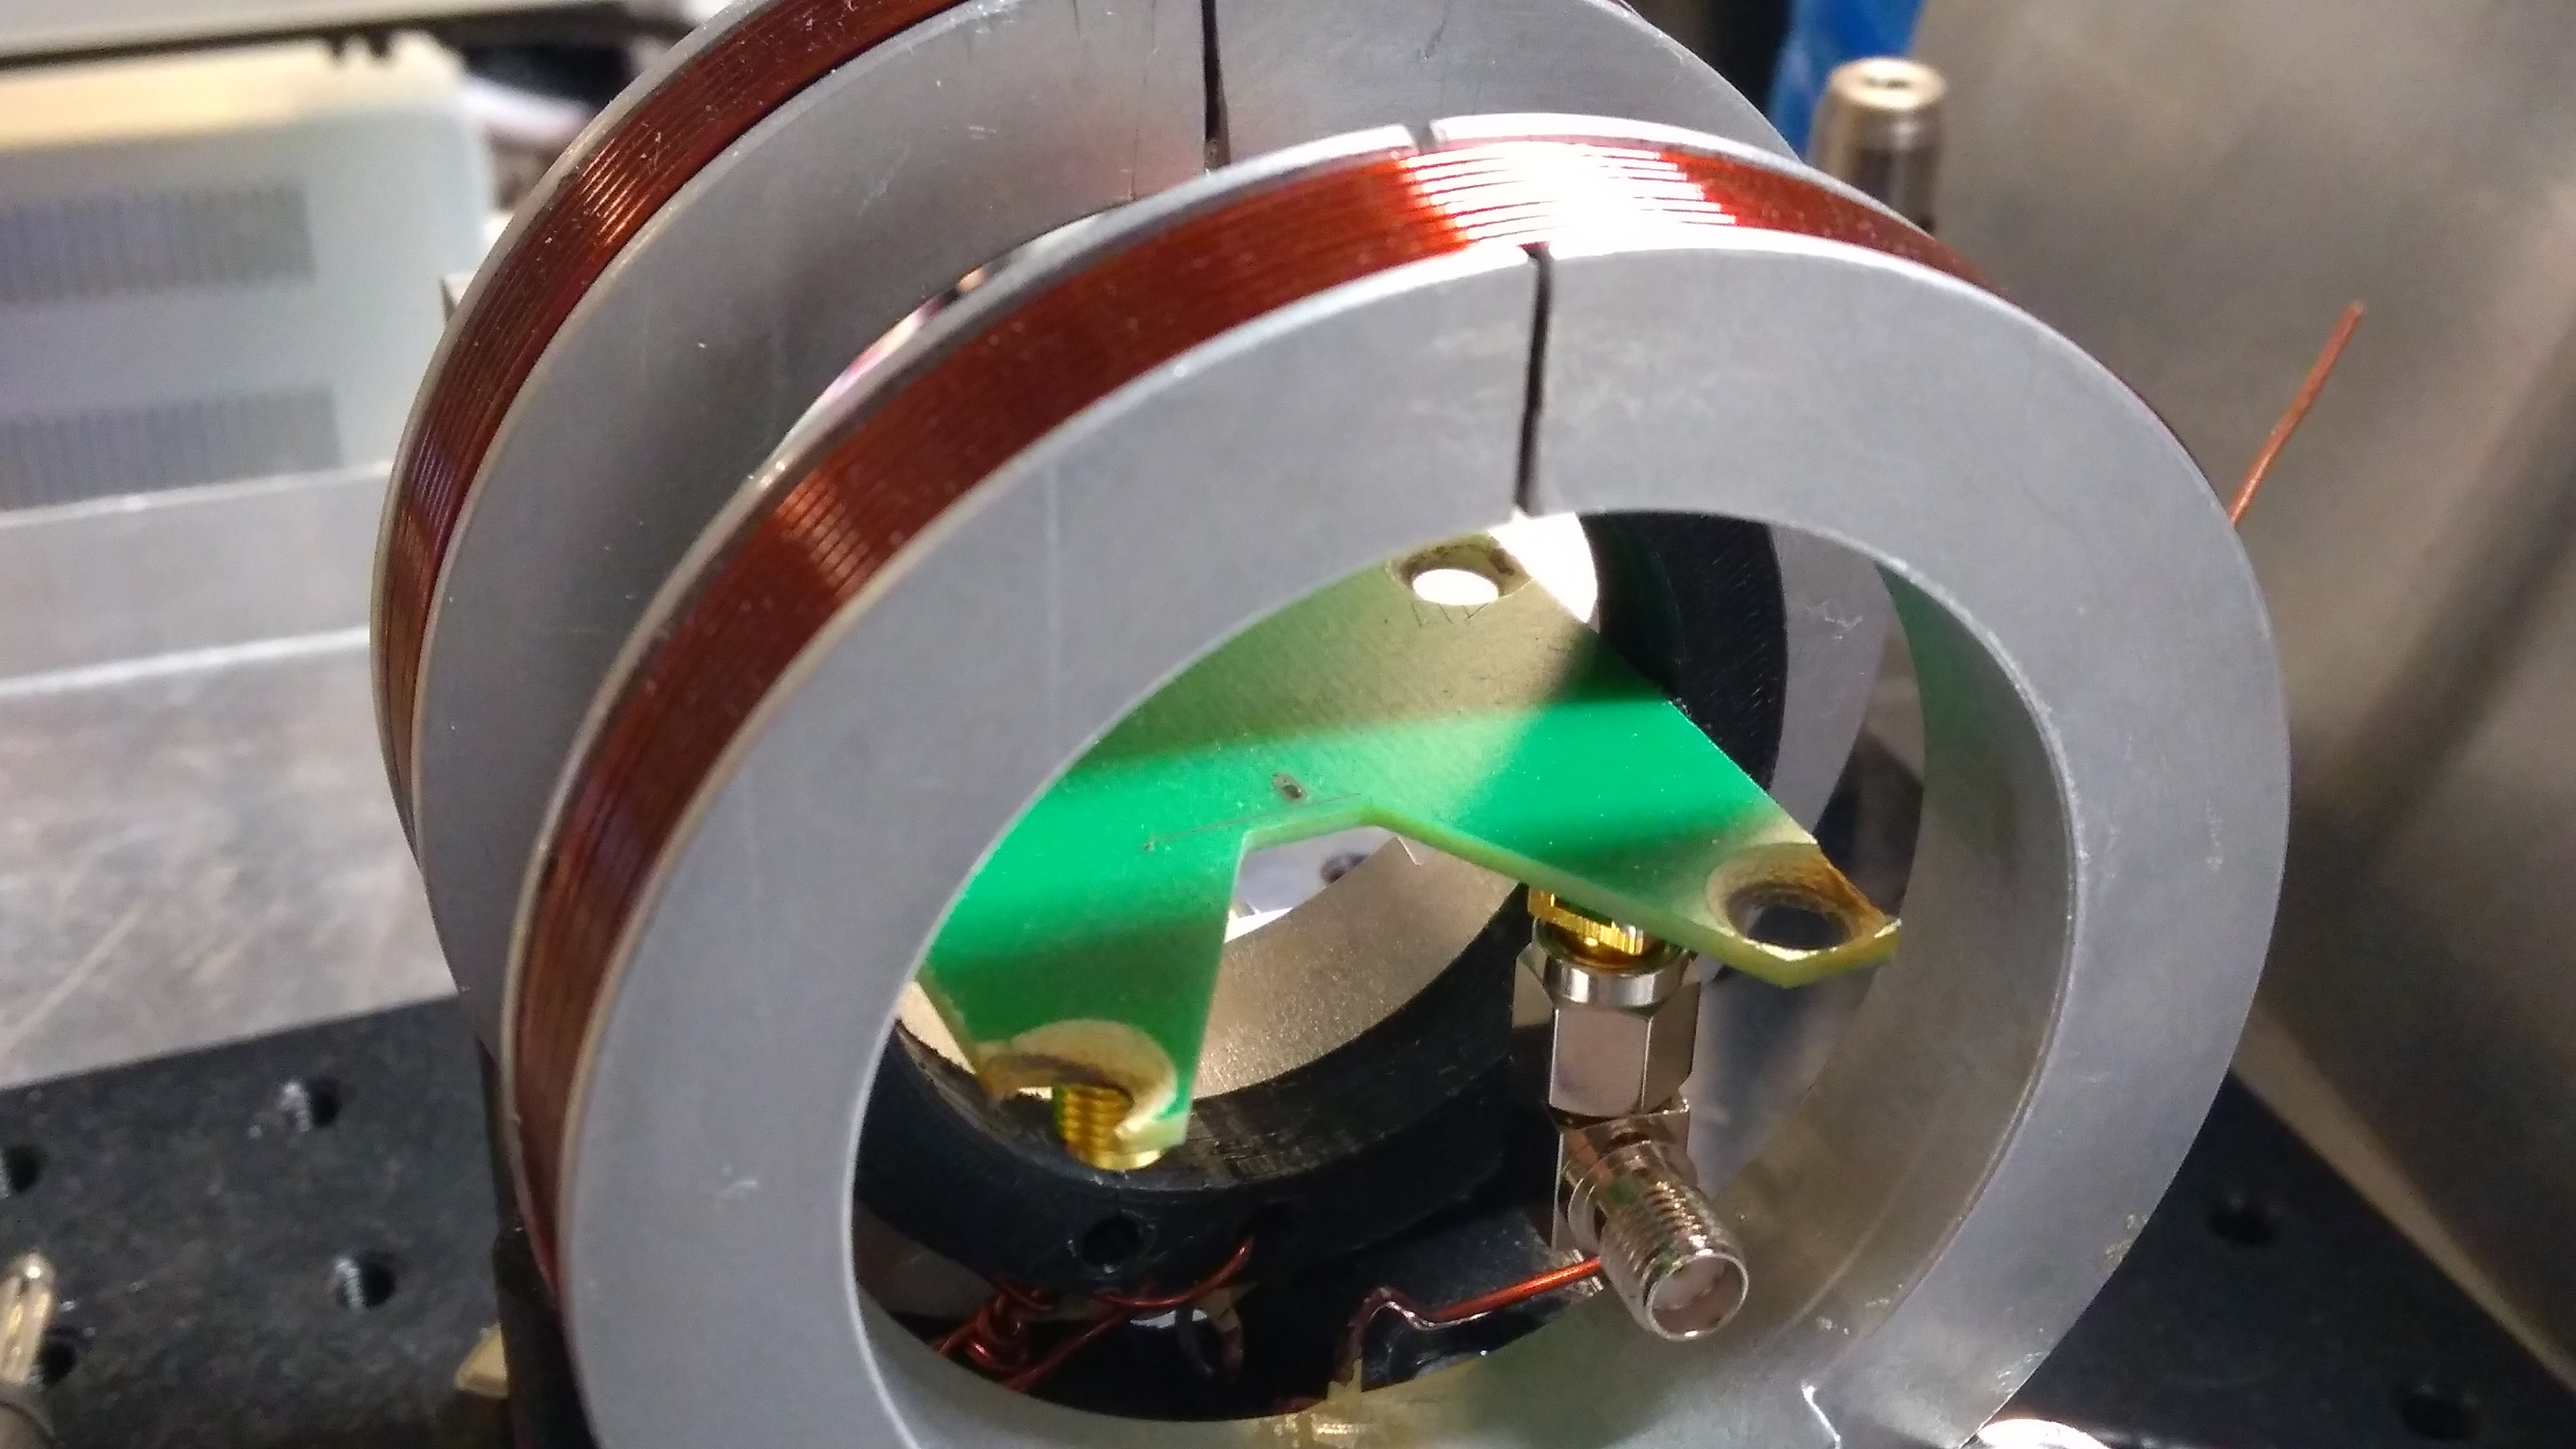
\includegraphics[width=\columnwidth]{figures/esrsetuppcb.jpg}
          \end{column}
        \end{columns}

        \begin{columns}
          \begin{column}{0.6\columnwidth}
            \begin{itemize}
              \item As sample we use the Koelsch radical ($\alpha,\gamma$-Bisdiphenylene-$\beta$-phenylallyl - BDPA)
              \item It has an unpaired spin $\to$ high spin density
              \item Excitation with microwave works at room temperature
              \item There is massive RF excitation background by radiated fields in our setup $\to$ differential measurements with and
                    without electron beam or at different distances to the modulated beam are required
            \end{itemize}
          \end{column}
          \begin{column}{0.4\columnwidth}
            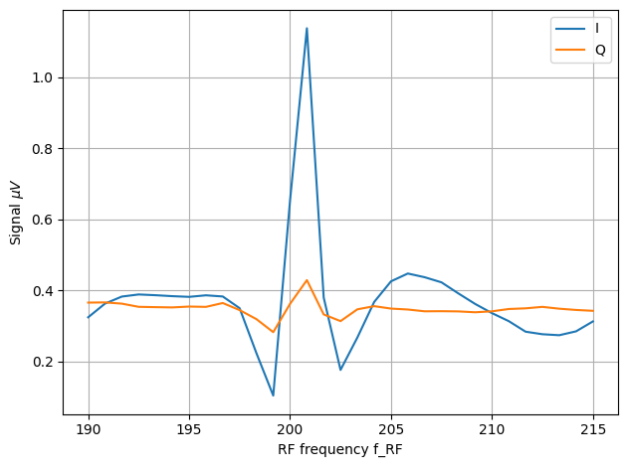
\includegraphics[width=\columnwidth]{figures/eprsignal.png}
          \end{column}
        \end{columns}
      \end{block}

      \begin{block}{\large Temperature dependence}
        We want to move to a cryogenic environment. This is done due to the small signal generated by the modulated electron beam.
        The thermal population of spin states is heavily temperature dependent:
        
        $$\frac{n_2}{n_1} = e^{-\frac{\Delta E}{k_B T}} = \left(e^{- \frac{\Delta E}{k_B}}\right)^\frac{1}{T}$$

        \vskip1ex
        \begin{columns}
          \begin{column}{0.4\columnwidth}
            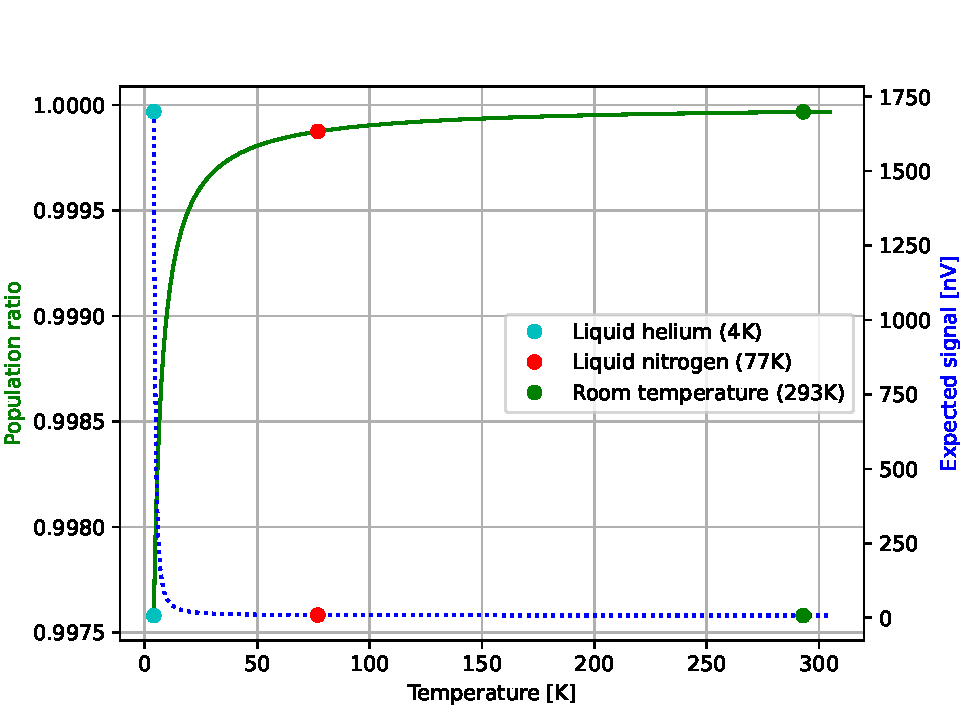
\includegraphics[width=\columnwidth]{figures/tempn2n1.pdf}
          \end{column}
          \begin{column}{0.6\columnwidth}
            \begin{itemize}
              \item Room temperature: \\ expect $22.9 nV$ signal, $185.83 \sqrt{Hz}$ SNR
              \item Moving to $77K$ (liquid nitrogen): \\ expect $89 nV$ signal, $1221.46 \sqrt{Hz}$ SNR \\ expected gain $\approx 4$, SNR gain $\approx 7.7$ \\ simple to realize, our choice
              \item Moving to $4K$ (liquid helium): \\ expect $1.7\mu V$ signal, $103163.45 \sqrt{Hz}$ SNR \\ expected gain $\approx 75$, SNR gain $\approx 649.5$ \\ challenging to realize
            \end{itemize}
          \end{column}
        \end{columns}
        \vskip1ex

        Averaging increases the SNR by $\sqrt{N}$ for N iterations. Doubling SNR of the system decreases the number of required averages by a factor of four. A gain of 4 decreases measurement time by a factor of 16,
        a gain of 650 would decrease measurement time by about half a million
      \end{block}

%%      \begin{block}{\large Contact}
%%          Thomas Spielauer \\ 
%%          Technische Universität Wien, Atominstitut \\ 
%%          thomas.spielauer@tuwien.ac.at
%%      \end{block}
    \end{column}

    % -------------------------------------------------------------

    \begin{column}{.49\linewidth}
      \begin{block}{\large Experimental setup}
        \begin{columns}
          \begin{column}{0.4\columnwidth}
            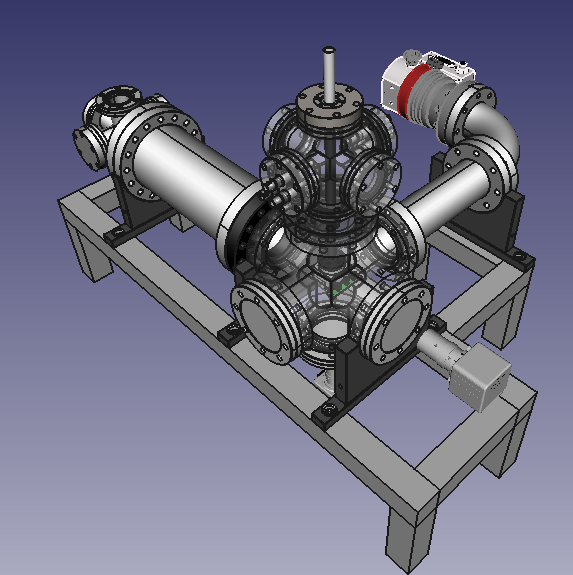
\includegraphics[width=\columnwidth]{figures/cryoquak02.png}
          \end{column}
          \begin{column}{0.6\columnwidth}
              \begin{itemize}
                \item The experiment runs in vacuum at $10^{-8}$ mbar or better
                \item As electron source we use a Barium-Strontium cathode, the beam is steered
                    by electrostatic beam deflection. The source provides $\geq 10 \mu A$ beam
                    current at up to $2.2 kV$ acceleration voltage.
                \item The beam modulation frequency is up to $\approx 250 MHz$
                \item Camera imaging from two directions of phosphor screens inside the
                    chamber and phosphor coated areas to determine and monitor beam
                    parameters.
                \item Cooling is done with liquid nitrogen from a reservoire on top
                    via a copper coldfinger through a teflon insulated steel pipe.
              \end{itemize}
          \end{column}
        \end{columns}
      \end{block}

      \begin{block}{\large Readout and radio frequency setup}
        \begin{columns}
          \begin{column}{0.6\columnwidth}
            \begin{itemize}
              \item We are using a carrier PCB thermally coupled to a copper coldfinger.
                    The PCB contains the microcoils as well as an RF impedance match,
                    copper areas and thermal vias to thermally couple to the coldfinger
                    and high voltage protection via an RF choke.
              \item We plan to use a second coil for reference measurements.
              \item The BDPA sample is positioned inside the microcoil (2 windings, $2.58$ x $1.14mm$
                    outer diameter, $1.5$ x $0.5mm$ sample area) in a milled pocket.
            \end{itemize}
          \end{column}
          \begin{column}{0.4\columnwidth}
            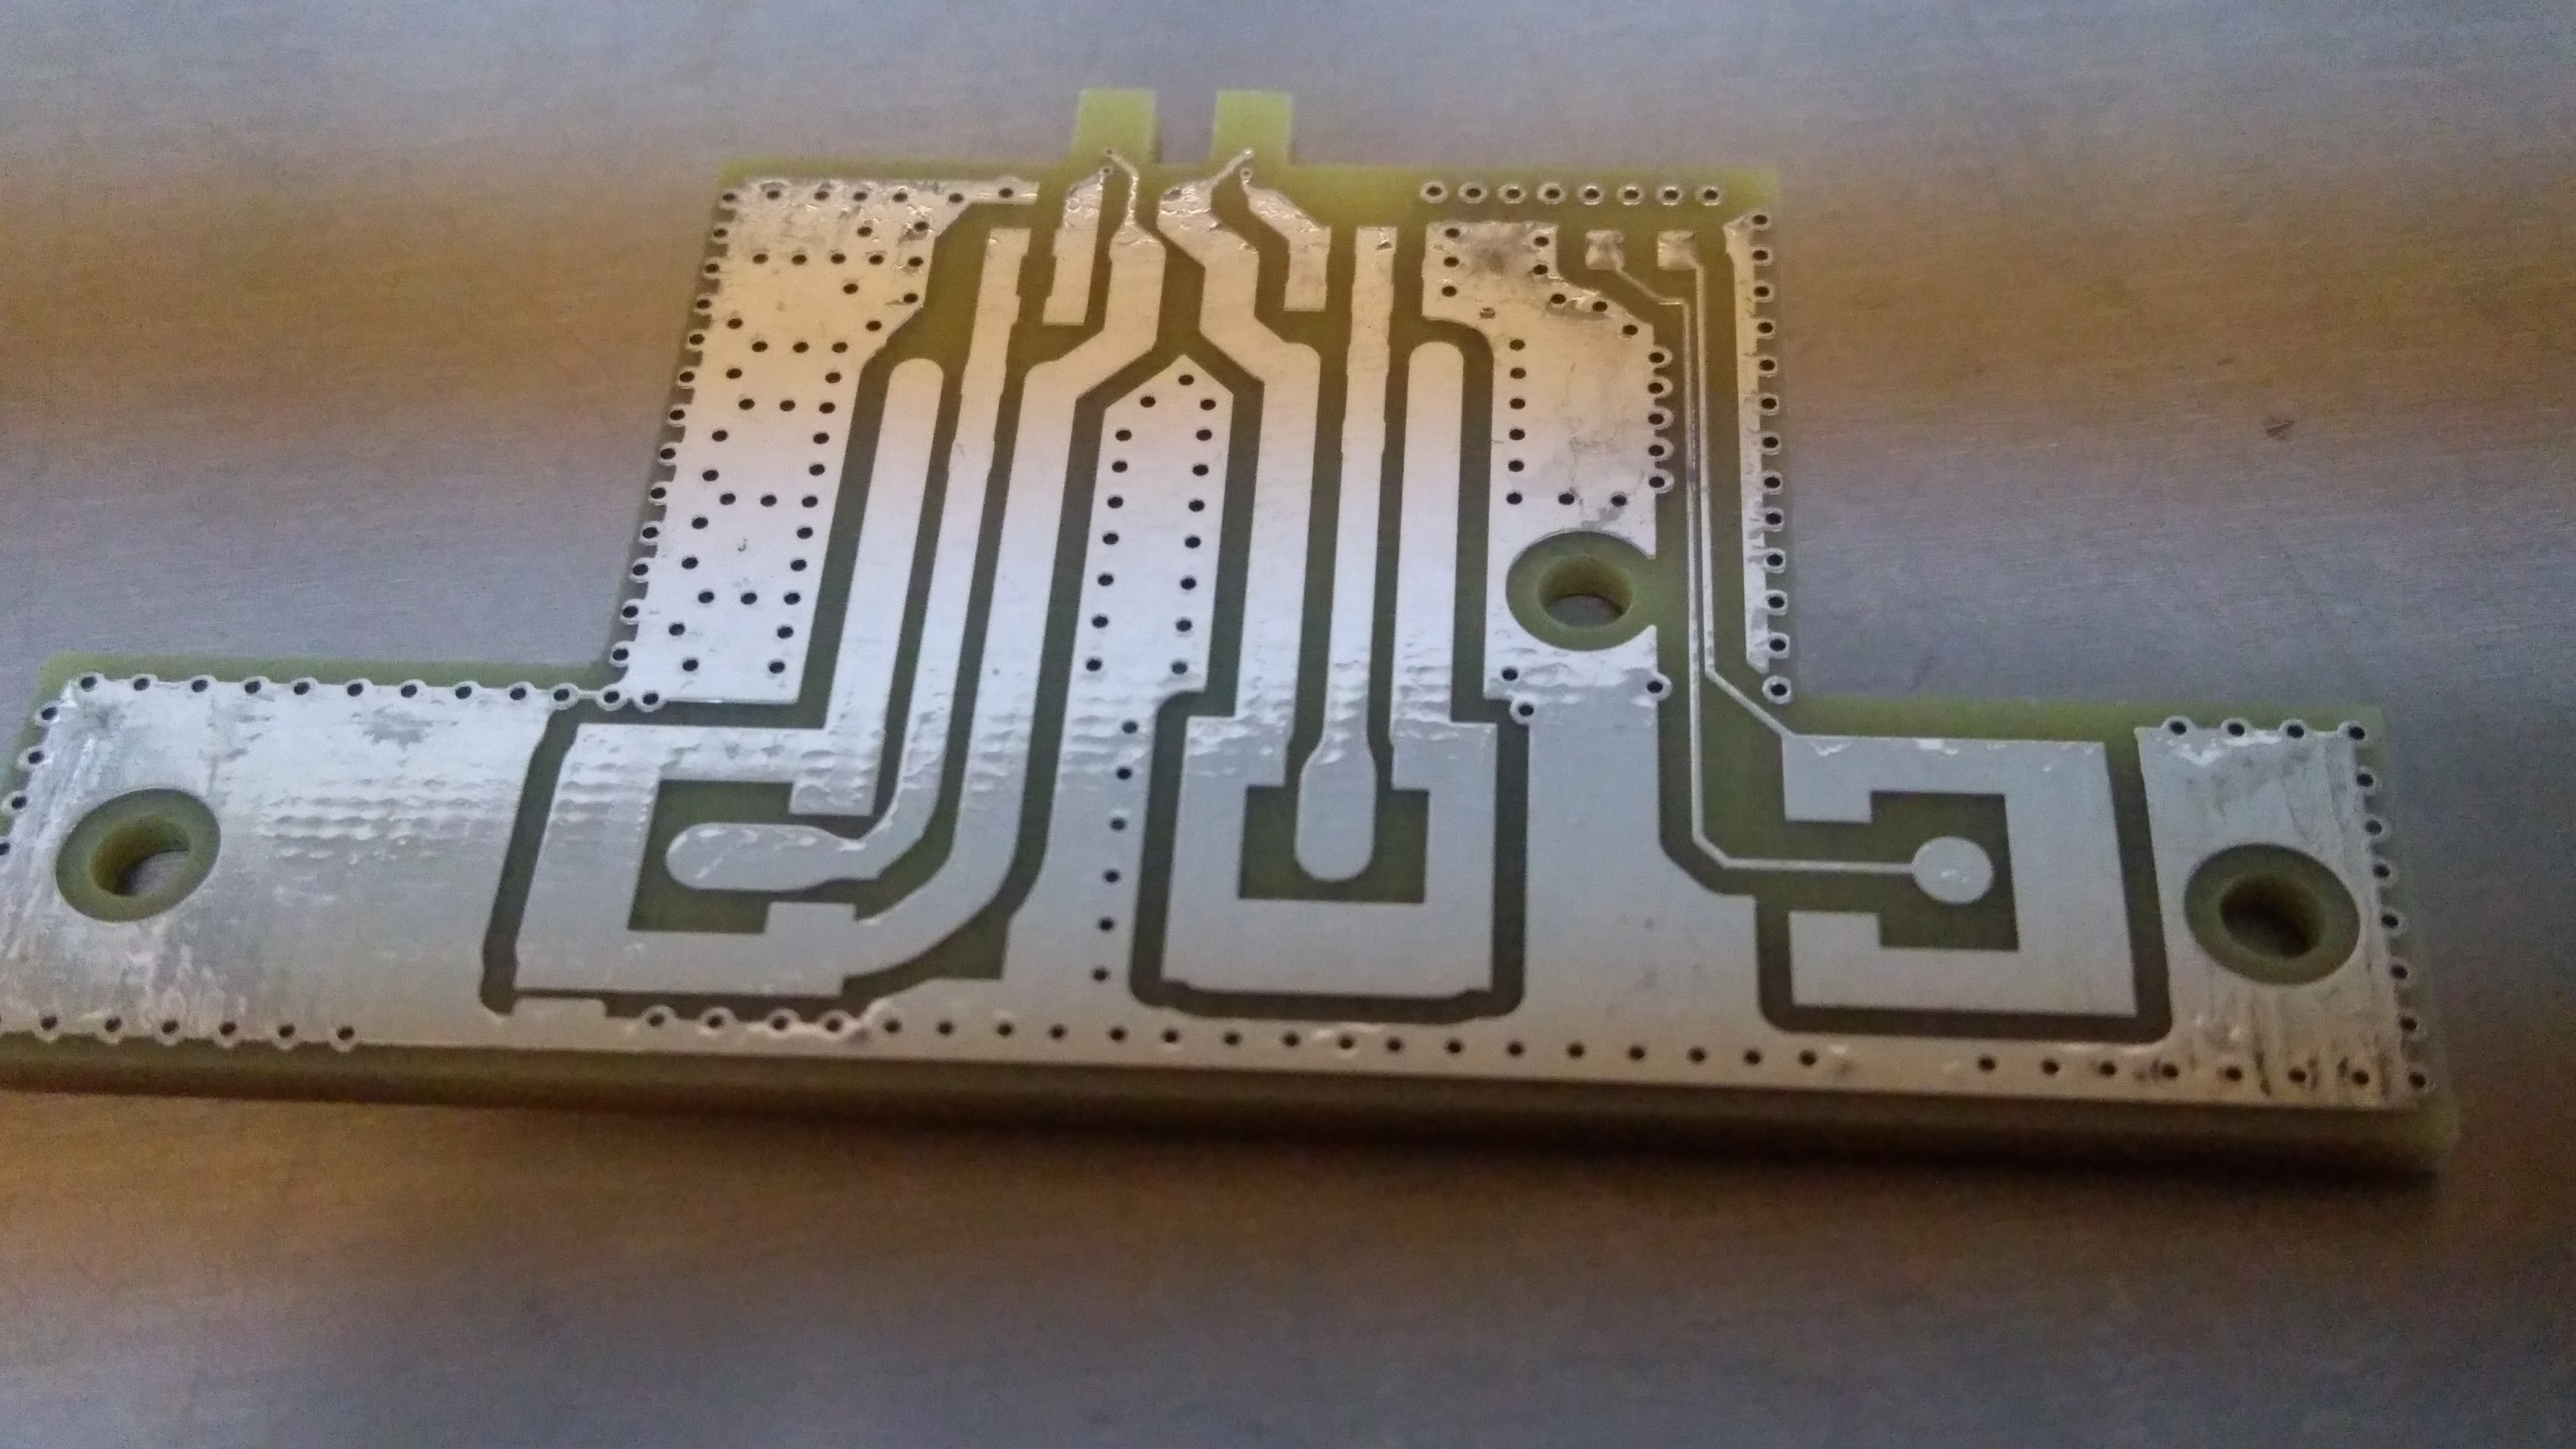
\includegraphics[width=\columnwidth]{figures/pcb01.jpg}

            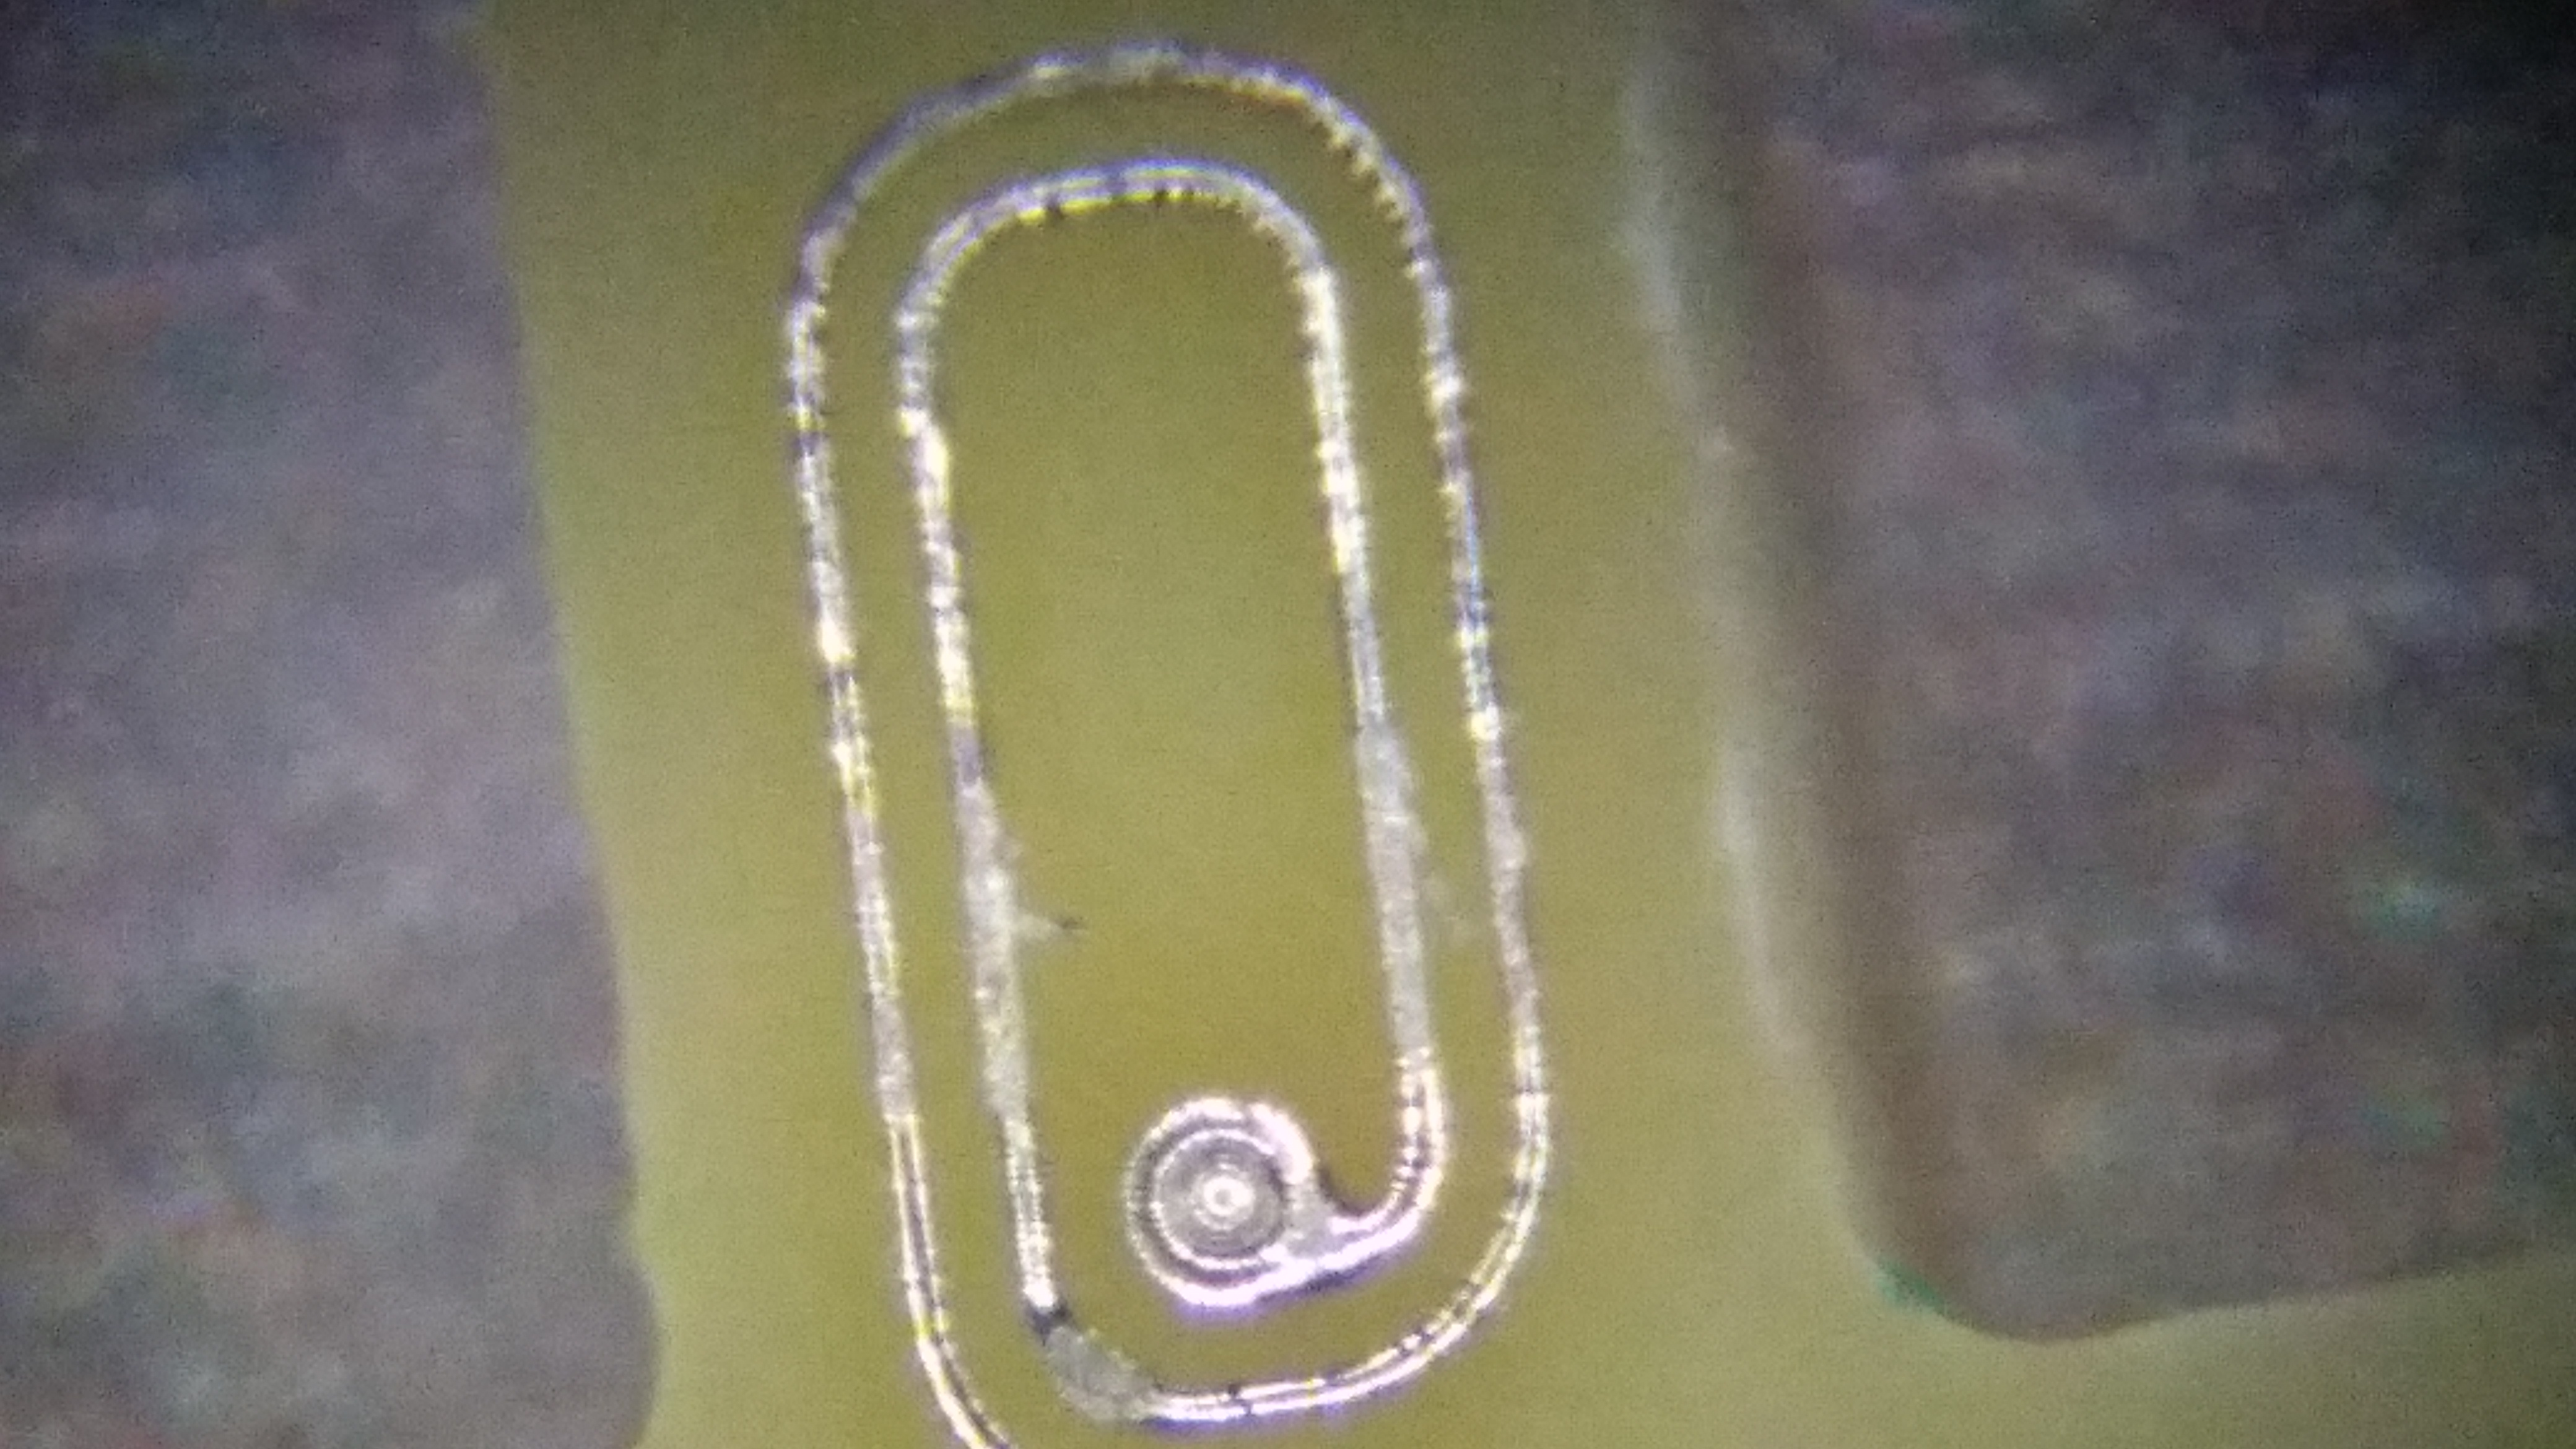
\includegraphics[width=\columnwidth]{figures/pcb02.jpg}
          \end{column}
        \end{columns}

        \begin{columns}
          \begin{column}{0.6\columnwidth}
            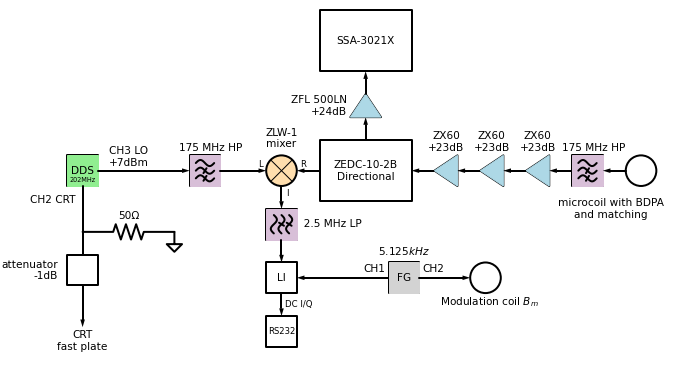
\includegraphics[width=\columnwidth]{figures/rfsetup.png}
          \end{column}
          \begin{column}{0.4\columnwidth}
            \begin{itemize}
              \item We are using two independent channels of an AD9959 based DDS for
                  local oscillator and beam deflection (excitation).
              \item Applying additional $5.123 kHz$ modulation field $B_m$ in
                  same direction as $B_0$
              \item Performing lock-in detection for better noise suppression
            \end{itemize}
          \end{column}
        \end{columns}
      \end{block}

      \begin{block}{\large First tests on test setup}
        We did some initial tests on our setup by simply cooling a PCB containing our
        BDPA sample in a liquid nitrogen bath.

        \begin{columns}
          \begin{column}{0.4\columnwidth}
            \begin{itemize}
              \item Excited using microwaves at various frequencies via a directional
                coupler as in a traditional EPR setup.
              \item Scanned $B_0$ field
              \item Compared amplitudes of maximum detected EPR signals
              \item Resonance frequency shifted
              \item About gain of 4 for signal amplitude
            \end{itemize}
          \end{column}
          \begin{column}{0.6\columnwidth}
            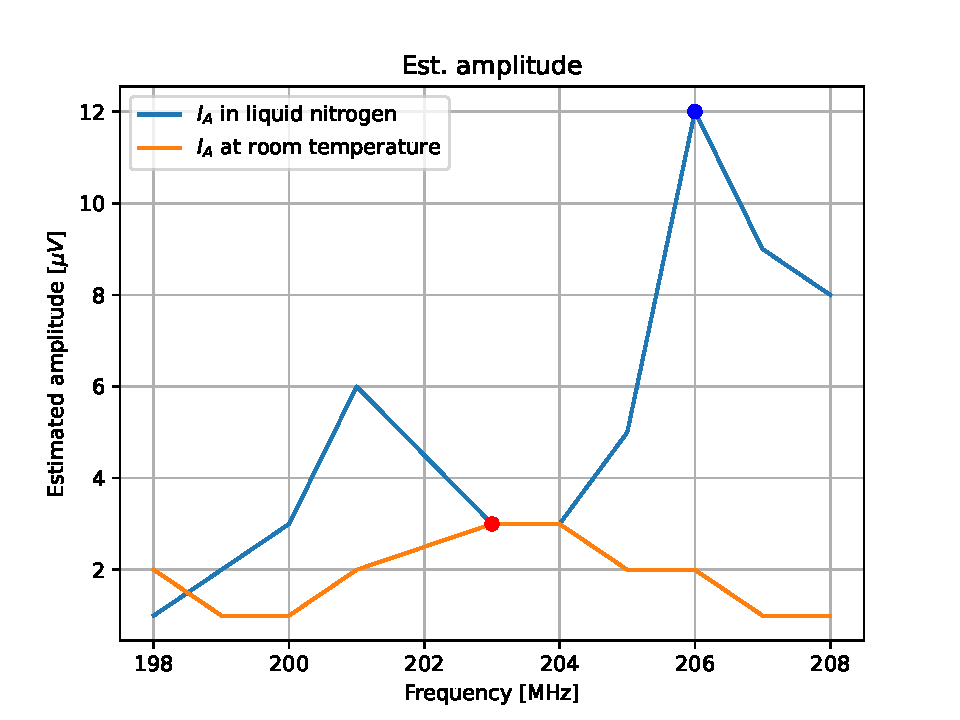
\includegraphics[width=\columnwidth]{figures/cryoamplitudes.pdf}
          \end{column}
        \end{columns}

        We saw the expected increase in signal amplitude as well as a shift of our
        impedance match that we have to compensate for.
      \end{block}

      \vskip4.5ex

      \begin{block}{\large References \& Acknowledgements}
        [1] D. Rätzel, D. Hartley, O. Schwartz, P. Haslinger, A Quantum
        Klystron - Controlling Quantum Systems with Modulated Electron Beams.
        \textit{Phys. Rev. Research 3, 023247 (2021)}
      \end{block}

    \end{column}

  \end{columns}

\end{frame}
\end{document}
